% Options for packages loaded elsewhere
% Options for packages loaded elsewhere
\PassOptionsToPackage{unicode}{hyperref}
\PassOptionsToPackage{hyphens}{url}
\PassOptionsToPackage{dvipsnames,svgnames,x11names}{xcolor}
%
\documentclass[
  letterpaper,
  DIV=11,
  numbers=noendperiod]{scrartcl}
\usepackage{xcolor}
\usepackage{amsmath,amssymb}
\setcounter{secnumdepth}{-\maxdimen} % remove section numbering
\usepackage{iftex}
\ifPDFTeX
  \usepackage[T1]{fontenc}
  \usepackage[utf8]{inputenc}
  \usepackage{textcomp} % provide euro and other symbols
\else % if luatex or xetex
  \usepackage{unicode-math} % this also loads fontspec
  \defaultfontfeatures{Scale=MatchLowercase}
  \defaultfontfeatures[\rmfamily]{Ligatures=TeX,Scale=1}
\fi
\usepackage{lmodern}
\ifPDFTeX\else
  % xetex/luatex font selection
\fi
% Use upquote if available, for straight quotes in verbatim environments
\IfFileExists{upquote.sty}{\usepackage{upquote}}{}
\IfFileExists{microtype.sty}{% use microtype if available
  \usepackage[]{microtype}
  \UseMicrotypeSet[protrusion]{basicmath} % disable protrusion for tt fonts
}{}
\makeatletter
\@ifundefined{KOMAClassName}{% if non-KOMA class
  \IfFileExists{parskip.sty}{%
    \usepackage{parskip}
  }{% else
    \setlength{\parindent}{0pt}
    \setlength{\parskip}{6pt plus 2pt minus 1pt}}
}{% if KOMA class
  \KOMAoptions{parskip=half}}
\makeatother
% Make \paragraph and \subparagraph free-standing
\makeatletter
\ifx\paragraph\undefined\else
  \let\oldparagraph\paragraph
  \renewcommand{\paragraph}{
    \@ifstar
      \xxxParagraphStar
      \xxxParagraphNoStar
  }
  \newcommand{\xxxParagraphStar}[1]{\oldparagraph*{#1}\mbox{}}
  \newcommand{\xxxParagraphNoStar}[1]{\oldparagraph{#1}\mbox{}}
\fi
\ifx\subparagraph\undefined\else
  \let\oldsubparagraph\subparagraph
  \renewcommand{\subparagraph}{
    \@ifstar
      \xxxSubParagraphStar
      \xxxSubParagraphNoStar
  }
  \newcommand{\xxxSubParagraphStar}[1]{\oldsubparagraph*{#1}\mbox{}}
  \newcommand{\xxxSubParagraphNoStar}[1]{\oldsubparagraph{#1}\mbox{}}
\fi
\makeatother

\usepackage{color}
\usepackage{fancyvrb}
\newcommand{\VerbBar}{|}
\newcommand{\VERB}{\Verb[commandchars=\\\{\}]}
\DefineVerbatimEnvironment{Highlighting}{Verbatim}{commandchars=\\\{\}}
% Add ',fontsize=\small' for more characters per line
\usepackage{framed}
\definecolor{shadecolor}{RGB}{241,243,245}
\newenvironment{Shaded}{\begin{snugshade}}{\end{snugshade}}
\newcommand{\AlertTok}[1]{\textcolor[rgb]{0.68,0.00,0.00}{#1}}
\newcommand{\AnnotationTok}[1]{\textcolor[rgb]{0.37,0.37,0.37}{#1}}
\newcommand{\AttributeTok}[1]{\textcolor[rgb]{0.40,0.45,0.13}{#1}}
\newcommand{\BaseNTok}[1]{\textcolor[rgb]{0.68,0.00,0.00}{#1}}
\newcommand{\BuiltInTok}[1]{\textcolor[rgb]{0.00,0.23,0.31}{#1}}
\newcommand{\CharTok}[1]{\textcolor[rgb]{0.13,0.47,0.30}{#1}}
\newcommand{\CommentTok}[1]{\textcolor[rgb]{0.37,0.37,0.37}{#1}}
\newcommand{\CommentVarTok}[1]{\textcolor[rgb]{0.37,0.37,0.37}{\textit{#1}}}
\newcommand{\ConstantTok}[1]{\textcolor[rgb]{0.56,0.35,0.01}{#1}}
\newcommand{\ControlFlowTok}[1]{\textcolor[rgb]{0.00,0.23,0.31}{\textbf{#1}}}
\newcommand{\DataTypeTok}[1]{\textcolor[rgb]{0.68,0.00,0.00}{#1}}
\newcommand{\DecValTok}[1]{\textcolor[rgb]{0.68,0.00,0.00}{#1}}
\newcommand{\DocumentationTok}[1]{\textcolor[rgb]{0.37,0.37,0.37}{\textit{#1}}}
\newcommand{\ErrorTok}[1]{\textcolor[rgb]{0.68,0.00,0.00}{#1}}
\newcommand{\ExtensionTok}[1]{\textcolor[rgb]{0.00,0.23,0.31}{#1}}
\newcommand{\FloatTok}[1]{\textcolor[rgb]{0.68,0.00,0.00}{#1}}
\newcommand{\FunctionTok}[1]{\textcolor[rgb]{0.28,0.35,0.67}{#1}}
\newcommand{\ImportTok}[1]{\textcolor[rgb]{0.00,0.46,0.62}{#1}}
\newcommand{\InformationTok}[1]{\textcolor[rgb]{0.37,0.37,0.37}{#1}}
\newcommand{\KeywordTok}[1]{\textcolor[rgb]{0.00,0.23,0.31}{\textbf{#1}}}
\newcommand{\NormalTok}[1]{\textcolor[rgb]{0.00,0.23,0.31}{#1}}
\newcommand{\OperatorTok}[1]{\textcolor[rgb]{0.37,0.37,0.37}{#1}}
\newcommand{\OtherTok}[1]{\textcolor[rgb]{0.00,0.23,0.31}{#1}}
\newcommand{\PreprocessorTok}[1]{\textcolor[rgb]{0.68,0.00,0.00}{#1}}
\newcommand{\RegionMarkerTok}[1]{\textcolor[rgb]{0.00,0.23,0.31}{#1}}
\newcommand{\SpecialCharTok}[1]{\textcolor[rgb]{0.37,0.37,0.37}{#1}}
\newcommand{\SpecialStringTok}[1]{\textcolor[rgb]{0.13,0.47,0.30}{#1}}
\newcommand{\StringTok}[1]{\textcolor[rgb]{0.13,0.47,0.30}{#1}}
\newcommand{\VariableTok}[1]{\textcolor[rgb]{0.07,0.07,0.07}{#1}}
\newcommand{\VerbatimStringTok}[1]{\textcolor[rgb]{0.13,0.47,0.30}{#1}}
\newcommand{\WarningTok}[1]{\textcolor[rgb]{0.37,0.37,0.37}{\textit{#1}}}

\usepackage{longtable,booktabs,array}
\usepackage{calc} % for calculating minipage widths
% Correct order of tables after \paragraph or \subparagraph
\usepackage{etoolbox}
\makeatletter
\patchcmd\longtable{\par}{\if@noskipsec\mbox{}\fi\par}{}{}
\makeatother
% Allow footnotes in longtable head/foot
\IfFileExists{footnotehyper.sty}{\usepackage{footnotehyper}}{\usepackage{footnote}}
\makesavenoteenv{longtable}
\usepackage{graphicx}
\makeatletter
\newsavebox\pandoc@box
\newcommand*\pandocbounded[1]{% scales image to fit in text height/width
  \sbox\pandoc@box{#1}%
  \Gscale@div\@tempa{\textheight}{\dimexpr\ht\pandoc@box+\dp\pandoc@box\relax}%
  \Gscale@div\@tempb{\linewidth}{\wd\pandoc@box}%
  \ifdim\@tempb\p@<\@tempa\p@\let\@tempa\@tempb\fi% select the smaller of both
  \ifdim\@tempa\p@<\p@\scalebox{\@tempa}{\usebox\pandoc@box}%
  \else\usebox{\pandoc@box}%
  \fi%
}
% Set default figure placement to htbp
\def\fps@figure{htbp}
\makeatother





\setlength{\emergencystretch}{3em} % prevent overfull lines

\providecommand{\tightlist}{%
  \setlength{\itemsep}{0pt}\setlength{\parskip}{0pt}}



 


\KOMAoption{captions}{tableheading}
\makeatletter
\@ifpackageloaded{caption}{}{\usepackage{caption}}
\AtBeginDocument{%
\ifdefined\contentsname
  \renewcommand*\contentsname{Table of contents}
\else
  \newcommand\contentsname{Table of contents}
\fi
\ifdefined\listfigurename
  \renewcommand*\listfigurename{List of Figures}
\else
  \newcommand\listfigurename{List of Figures}
\fi
\ifdefined\listtablename
  \renewcommand*\listtablename{List of Tables}
\else
  \newcommand\listtablename{List of Tables}
\fi
\ifdefined\figurename
  \renewcommand*\figurename{Figure}
\else
  \newcommand\figurename{Figure}
\fi
\ifdefined\tablename
  \renewcommand*\tablename{Table}
\else
  \newcommand\tablename{Table}
\fi
}
\@ifpackageloaded{float}{}{\usepackage{float}}
\floatstyle{ruled}
\@ifundefined{c@chapter}{\newfloat{codelisting}{h}{lop}}{\newfloat{codelisting}{h}{lop}[chapter]}
\floatname{codelisting}{Listing}
\newcommand*\listoflistings{\listof{codelisting}{List of Listings}}
\makeatother
\makeatletter
\makeatother
\makeatletter
\@ifpackageloaded{caption}{}{\usepackage{caption}}
\@ifpackageloaded{subcaption}{}{\usepackage{subcaption}}
\makeatother
\usepackage{bookmark}
\IfFileExists{xurl.sty}{\usepackage{xurl}}{} % add URL line breaks if available
\urlstyle{same}
\hypersetup{
  pdftitle={Lab Assignment \#7},
  pdfauthor={Math 437 - Modern Data Analysis},
  colorlinks=true,
  linkcolor={blue},
  filecolor={Maroon},
  citecolor={Blue},
  urlcolor={Blue},
  pdfcreator={LaTeX via pandoc}}


\title{Lab Assignment \#7}
\author{Math 437 - Modern Data Analysis}
\date{}
\begin{document}
\maketitle


80-90\% of modeling work is getting the data in a form suitable for
modeling. Much of that work is intelligent data wrangling. Much of that
``intelligent'' is informed by good exploratory data analysis.

In this lab will start exploratory data analysis on the
\texttt{RateMyProfessor} dataset.

Recall that a data dictionary for this dataset can be found at the
\href{https://github.com/murrayds/aa_rmp/tree/master/data}{original data
source}.

\begin{Shaded}
\begin{Highlighting}[]
\NormalTok{here}\SpecialCharTok{::}\FunctionTok{i\_am}\NormalTok{(}\StringTok{"Labs/Lab07.qmd"}\NormalTok{)}

\CommentTok{\# just load all the main tidyverse packages at once}
\CommentTok{\# including dplyr and ggplot2}
\FunctionTok{library}\NormalTok{(tidyverse)}
\FunctionTok{library}\NormalTok{(tidymodels)}

\CommentTok{\# load data}
\NormalTok{RateMyProfessor }\OtherTok{\textless{}{-}}\NormalTok{ readr}\SpecialCharTok{::}\FunctionTok{read\_csv}\NormalTok{(here}\SpecialCharTok{::}\FunctionTok{here}\NormalTok{(}\StringTok{"C:/Users/aocho/Downloads/RateMyProfessor.csv"}\NormalTok{))}

\CommentTok{\# Use my training/holdout split}
\FunctionTok{set.seed}\NormalTok{(}\DecValTok{230}\NormalTok{)}
\NormalTok{RMP\_split }\OtherTok{\textless{}{-}} \FunctionTok{initial\_split}\NormalTok{(RateMyProfessor, }\AttributeTok{prop =} \FloatTok{0.80}\NormalTok{)}
\NormalTok{RMP\_train }\OtherTok{\textless{}{-}} \FunctionTok{training}\NormalTok{(RMP\_split)}
\CommentTok{\# we\textquotesingle{}re not modeling here, ignore the test set}
\CommentTok{\#RMP\_test \textless{}{-} testing(RMP\_split)}
\FunctionTok{head}\NormalTok{(RateMyProfessor)}
\end{Highlighting}
\end{Shaded}

\begin{verbatim}
# A tibble: 6 x 15
     id overall difficulty review_count interest mentions_accent mentions_ta
  <dbl>   <dbl>      <dbl>        <dbl>    <dbl> <lgl>           <lgl>      
1    59    4.25       2.75            4     5    FALSE           FALSE      
2   107    3.44       3.78            9     4.11 FALSE           FALSE      
3   121    3.78       3.56            9     3.5  FALSE           FALSE      
4   124    3.5        3.5             4     3.75 FALSE           FALSE      
5   150    2.75       3.5             4     3    FALSE           FALSE      
6   154    1.6        4.6            10     3.67 FALSE           FALSE      
# i 8 more variables: hotness <chr>, scientific_age <dbl>, rank <chr>,
#   gender <chr>, race <chr>, discipline <chr>, uni_type <chr>,
#   uni_control <chr>
\end{verbatim}

This lab assignment is worth a total of \textbf{15 points}.

\textbf{REMINDER}: Explore \emph{only} the \texttt{RMP\_train} dataset
in this lab.

\subsection{Problem 1: Univariate Exploration (3 pts
total)}\label{problem-1-univariate-exploration-3-pts-total}

Typically, the first thing we want to do is understand the context of
our data: What are we actually trying to predict? Why? How is the model
going to be used? What do we suspect needs to be included in the model?
Is there anything that shouldn't be included (for practical and/or
ethical reasons)?

Typically, the second thing we want to do is split into a training and a
holdout set, so that information from your holdout set doesn't ``leak
into'' your exploration of the data. We did this in the chunk above.

Then we start our exploratory data analysis on the training set by
exploring the response variable. In this case, we have chosen
\texttt{overall} as our response. We're looking for three big things:

\begin{itemize}
\tightlist
\item
  How many values are missing? Is there a pattern to the missingness?
\item
  Does the distribution of values make real-world sense? Does it match
  our expectations?
\item
  What do we have to watch out for when modeling?
\end{itemize}

\subsubsection{Part a (Explanation: 1
pt)}\label{part-a-explanation-1-pt}

What would you expect the distribution of \texttt{overall} to look like?
Why? Consider center, variability, shape, and outliers, and try not to
write with too much technical jargon.

\paragraph{Solution}\label{solution}

Since overall is a student rating on a 1--5 scale, I'd expect most of
the values to be toward the higher end. Usually students are more likely
to leave reviews when they had a good experience, so I wouldn't be
surprised if the distribution is slightly skewed toward higher ratings.
I'd expect the center to be somewhere around 3.5 to 4. There should be
some spread, but I wouldn't expect extreme outliers since the rating
scale is capped between 1 and 5.

\subsubsection{Part b (Code: 1 pt)}\label{part-b-code-1-pt}

Using the \texttt{summarize} function, obtain the mean, standard
deviation, and five-number summary of \texttt{overall}.

\paragraph{Solution}\label{solution-1}

\begin{Shaded}
\begin{Highlighting}[]
\NormalTok{RMP\_train }\SpecialCharTok{|\textgreater{}}
  \FunctionTok{summarize}\NormalTok{(}
    \AttributeTok{mean =} \FunctionTok{mean}\NormalTok{(overall, }\AttributeTok{na.rm =} \ConstantTok{TRUE}\NormalTok{),}
    \AttributeTok{sd =} \FunctionTok{sd}\NormalTok{(overall, }\AttributeTok{na.rm =} \ConstantTok{TRUE}\NormalTok{),}
    \AttributeTok{min =} \FunctionTok{min}\NormalTok{(overall, }\AttributeTok{na.rm =} \ConstantTok{TRUE}\NormalTok{),}
    \AttributeTok{Q1 =} \FunctionTok{quantile}\NormalTok{(overall, }\FloatTok{0.25}\NormalTok{, }\AttributeTok{na.rm =} \ConstantTok{TRUE}\NormalTok{),}
    \AttributeTok{median =} \FunctionTok{median}\NormalTok{(overall, }\AttributeTok{na.rm =} \ConstantTok{TRUE}\NormalTok{),}
    \AttributeTok{Q3 =} \FunctionTok{quantile}\NormalTok{(overall, }\FloatTok{0.75}\NormalTok{, }\AttributeTok{na.rm =} \ConstantTok{TRUE}\NormalTok{),}
    \AttributeTok{max =} \FunctionTok{max}\NormalTok{(overall, }\AttributeTok{na.rm =} \ConstantTok{TRUE}\NormalTok{)}
\NormalTok{  )}
\end{Highlighting}
\end{Shaded}

\begin{verbatim}
# A tibble: 1 x 7
   mean    sd   min    Q1 median    Q3   max
  <dbl> <dbl> <dbl> <dbl>  <dbl> <dbl> <dbl>
1  3.52 0.934     1  2.86   3.64  4.29     5
\end{verbatim}

\subsubsection{Part c (Code: 1 pt)}\label{part-c-code-1-pt}

Using the \texttt{ggplot2} package, construct a histogram of the
distribution of \texttt{overall}. Play around with the \texttt{center}
and \texttt{binwidth} arguments until you get a graph where you have a
good idea of the shape of the distribution.

Since you are just exploring the data right now, I don't care too much
about getting the title or axis labels exactly right - as long as ``next
week you'' knows what you're graphing, I'm okay with it, but there
should be at least some minimal effort into making them informative.

\paragraph{Solution}\label{solution-2}

\begin{Shaded}
\begin{Highlighting}[]
\FunctionTok{ggplot}\NormalTok{(RMP\_train, }
       \AttributeTok{mapping =} \FunctionTok{aes}\NormalTok{(}\AttributeTok{x =}\NormalTok{ overall)}
\NormalTok{       ) }\SpecialCharTok{+}
  \FunctionTok{geom\_histogram}\NormalTok{(}\AttributeTok{binwidth =} \FloatTok{0.25}\NormalTok{,}
                 \AttributeTok{color =} \StringTok{"black"}\NormalTok{,}
                 \AttributeTok{fill =} \StringTok{"steelblue"}\NormalTok{) }\SpecialCharTok{+}
  \FunctionTok{labs}\NormalTok{(}
    \AttributeTok{title =} \StringTok{"Distribution of Overall Professor Ratings"}\NormalTok{,}
    \AttributeTok{x =} \StringTok{"Overall Rating"}\NormalTok{,}
    \AttributeTok{y =} \StringTok{"Count"}
\NormalTok{  )}
\end{Highlighting}
\end{Shaded}

\pandocbounded{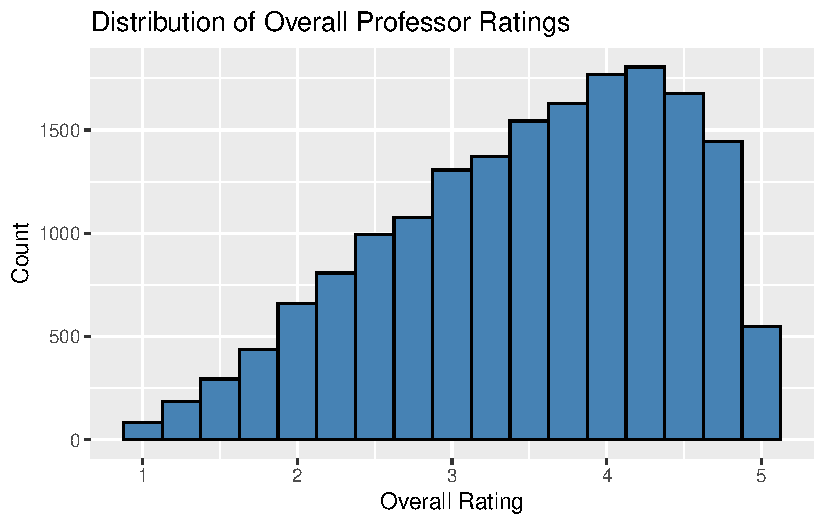
\includegraphics[keepaspectratio]{Lab07_files/figure-pdf/ggplot of overall-1.pdf}}

\subsubsection{Part d (Explanation: 1
pt)}\label{part-d-explanation-1-pt}

Write 1-2 sentences describing anything interesting that you notice
based on your summary and histogram. Some general questions to guide
what ``seems interesting'':

\begin{itemize}
\tightlist
\item
  Where do the ratings tend to be around? Does that match your
  expectation?
\item
  How spread out are the ratings around that center? Does that match
  your expectation?
\item
  Is there anything interesting about the shape of the distribution that
  would suggest further exploration (bimodality, extremely long
  left/right tail, etc.)?
\item
  Are there any outliers? If so, what professors do they correspond to,
  and is there anything interesting about those professors that warrants
  further exploration?
\end{itemize}

Try to write your answer using similar language to how you described
what you expected.

\paragraph{Solution}\label{solution-3}

Most of the ratings seem to be centered around the low 4s, which
honestly matches what I would expect since students usually rate
professors pretty generously. The spread isn't huge, and there aren't
many very low ratings, which makes the distribution slightly
left-skewed. There also don't appear to be extreme outliers since the
ratings are naturally limited between 1 and 5.

\subsection{Problem 2: Bivariate Exploration 1 (5 pts
total)}\label{problem-2-bivariate-exploration-1-5-pts-total}

Once we've looked at our response variable, we start investigating
potential explanatory/predictor variables. Some questions of interest
here include, in addition to the questions from Problem 1:

\begin{itemize}
\tightlist
\item
  What kind of relationship do we expect? Why? Is it shown in the data?
\item
  Are there any unusual (predictor, response) pairs? Any clusters of
  points that may indicate the influence of a third variable?
\item
  Are there any noticeable jumps/discontinuities, horizontal/vertical
  ``bands of points'', changes in trend/distribution, or similarly
  complex patterns that should be addressed when modeling?
\end{itemize}

\subsubsection{Part a (Explanation: 1
pt)}\label{part-a-explanation-1-pt-1}

Pick one of the following variables: \texttt{interest},
\texttt{review\_count}, or \texttt{scientific\_age}. \emph{Without doing
anything with the data}, explain what you would expect to happen to the
distribution of the \texttt{overall} rating as the value of that
variable increases, and explain why. Try not to write with too much
technical jargon.

\paragraph{Solution}\label{solution-4}

I would expect that as interest increases, the overall rating would also
tend to increase. If students find the class more interesting, they're
probably more likely to rate the professor higher. So I'd expect a
positive relationship between interest and overall rating.

\subsubsection{Part b (Code: 1 pt; Explanation: 1
pt)}\label{part-b-code-1-pt-explanation-1-pt}

Repeat Problem 1 for the variable you chose in Part a.

\paragraph{Solution}\label{solution-5}

\begin{Shaded}
\begin{Highlighting}[]
\NormalTok{RMP\_train }\SpecialCharTok{|\textgreater{}}
  \FunctionTok{summarize}\NormalTok{(}
    \AttributeTok{mean\_interest =} \FunctionTok{mean}\NormalTok{(interest, }\AttributeTok{na.rm =} \ConstantTok{TRUE}\NormalTok{),}
    \AttributeTok{sd\_interest   =} \FunctionTok{sd}\NormalTok{(interest, }\AttributeTok{na.rm =} \ConstantTok{TRUE}\NormalTok{),}
    \AttributeTok{min           =} \FunctionTok{min}\NormalTok{(interest, }\AttributeTok{na.rm =} \ConstantTok{TRUE}\NormalTok{),}
    \AttributeTok{Q1            =} \FunctionTok{quantile}\NormalTok{(interest, }\FloatTok{0.25}\NormalTok{, }\AttributeTok{na.rm =} \ConstantTok{TRUE}\NormalTok{),}
    \AttributeTok{median        =} \FunctionTok{median}\NormalTok{(interest, }\AttributeTok{na.rm =} \ConstantTok{TRUE}\NormalTok{),}
    \AttributeTok{Q3            =} \FunctionTok{quantile}\NormalTok{(interest, }\FloatTok{0.75}\NormalTok{, }\AttributeTok{na.rm =} \ConstantTok{TRUE}\NormalTok{),}
    \AttributeTok{max           =} \FunctionTok{max}\NormalTok{(interest, }\AttributeTok{na.rm =} \ConstantTok{TRUE}\NormalTok{)}
\NormalTok{  )}
\end{Highlighting}
\end{Shaded}

\begin{verbatim}
# A tibble: 1 x 7
  mean_interest sd_interest   min    Q1 median    Q3   max
          <dbl>       <dbl> <dbl> <dbl>  <dbl> <dbl> <dbl>
1          3.42       0.702     1     3   3.45     4     5
\end{verbatim}

\begin{Shaded}
\begin{Highlighting}[]
\CommentTok{\#histogram plot}
\FunctionTok{ggplot}\NormalTok{(RMP\_train,}
       \AttributeTok{mapping =} \FunctionTok{aes}\NormalTok{(}\AttributeTok{x =}\NormalTok{ interest)}
\NormalTok{       ) }\SpecialCharTok{+}
  \FunctionTok{geom\_histogram}\NormalTok{(}\AttributeTok{binwidth =} \FloatTok{0.25}\NormalTok{,}
                 \AttributeTok{fill =} \StringTok{"steelblue"}\NormalTok{,}
                 \AttributeTok{color =} \StringTok{"black"}\NormalTok{) }\SpecialCharTok{+}
  \FunctionTok{labs}\NormalTok{(}
    \AttributeTok{title =} \StringTok{"Distribution of Interest Ratings"}\NormalTok{,}
    \AttributeTok{x =} \StringTok{"Interest"}\NormalTok{,}
    \AttributeTok{y =} \StringTok{"Count"}
\NormalTok{  )}
\end{Highlighting}
\end{Shaded}

\pandocbounded{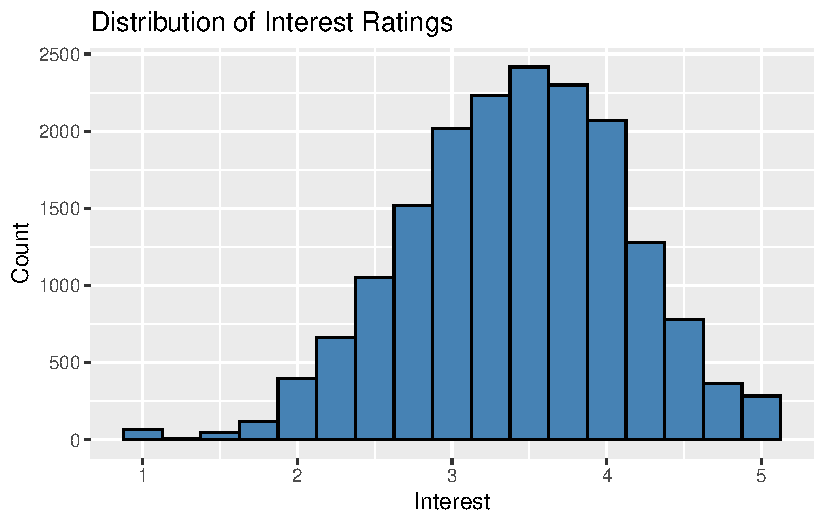
\includegraphics[keepaspectratio]{Lab07_files/figure-pdf/summurize function on interest and ggplot-1.pdf}}

Explanation: The interest ratings are centered around about 3.4 to 3.5,
with most values falling between 3 and 4. The distribution looks fairly
symmetric and not heavily skewed in either direction. There are a few
lower ratings near 1, but most of the data is concentrated in the middle
range, which makes sense since students probably rate classes as
moderately interesting rather than extremely boring or extremely
amazing.

\subsubsection{Part c (Code: 1 pt)}\label{part-c-code-1-pt-1}

Create a scatterplot showing the relationship between that variable and
\texttt{overall}. If the relationship looks approximately linear, add a
least-squares regression line (\texttt{method\ =\ "lm"}). If the
relationship looks nonlinear, add a local regression curve
(\texttt{method\ =\ "loess"}). If you can't tell (or the relationship is
very weak), add at least one of the two.

It's likely that with over 17,000 professors, this plot will be very
messy and there will be lots of overlap. You may want to use
\texttt{geom\_point(alpha\ =\ 0.1)} to make points with more professors
darker rather than using \texttt{geom\_jitter()} to remove the overlap.

\paragraph{Solution}\label{solution-6}

\begin{Shaded}
\begin{Highlighting}[]
\FunctionTok{ggplot}\NormalTok{(RMP\_train,}
       \AttributeTok{mapping =} \FunctionTok{aes}\NormalTok{(}\AttributeTok{x =}\NormalTok{ interest, }\AttributeTok{y =}\NormalTok{ overall)}
\NormalTok{       ) }\SpecialCharTok{+}
  \FunctionTok{geom\_point}\NormalTok{(}\AttributeTok{alpha =} \FloatTok{0.1}\NormalTok{,}
             \AttributeTok{color =} \StringTok{"steelblue"}\NormalTok{) }\SpecialCharTok{+}
  \FunctionTok{geom\_smooth}\NormalTok{(}\AttributeTok{method =} \StringTok{"lm"}\NormalTok{,}
              \AttributeTok{se =} \ConstantTok{FALSE}\NormalTok{,}
              \AttributeTok{color =} \StringTok{"darkred"}\NormalTok{) }\SpecialCharTok{+}
  \FunctionTok{labs}\NormalTok{(}
    \AttributeTok{title =} \StringTok{"Interest vs Overall Rating"}\NormalTok{,}
    \AttributeTok{x =} \StringTok{"Interest"}\NormalTok{,}
    \AttributeTok{y =} \StringTok{"Overall Rating"}
\NormalTok{  )}
\end{Highlighting}
\end{Shaded}

\begin{verbatim}
`geom_smooth()` using formula = 'y ~ x'
\end{verbatim}

\pandocbounded{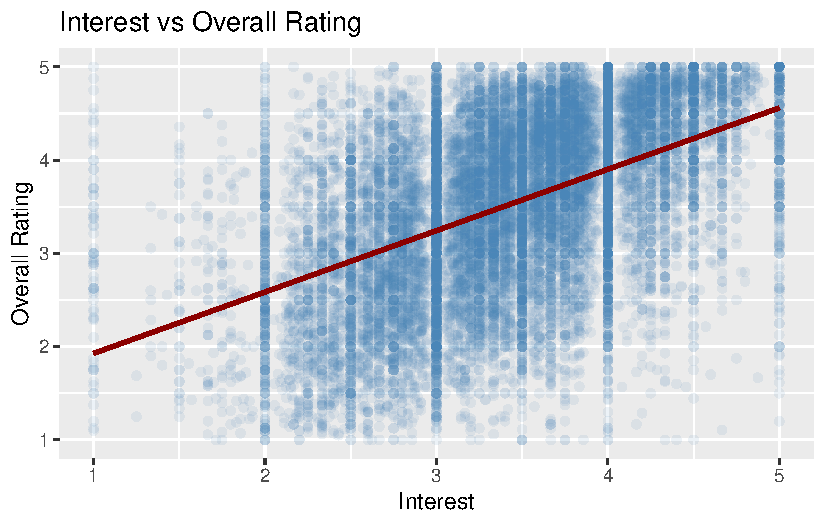
\includegraphics[keepaspectratio]{Lab07_files/figure-pdf/scatter plot of overall vs interest-1.pdf}}

\subsubsection{Part d (Explanation: 1
pt)}\label{part-d-explanation-1-pt-1}

Write 1-2 sentences describing anything interesting that you notice
based on the scatterplot. Try to address the questions suggested at the
beginning of this problem and refer to what you expected to see in Part
b.

\paragraph{Solution}\label{solution-7}

There is a noticeable upward trend between interest and overall rating,
which is what I expected. The relationship looks roughly linear, and
although the plot is messy due to the large number of observations, the
positive association is still clear.

\subsection{Problem 3: Bivariate Exploration 2 (5 pts
total)}\label{problem-3-bivariate-exploration-2-5-pts-total}

\subsubsection{Part a (Explanation: 1
pt)}\label{part-a-explanation-1-pt-2}

Choose any categorical or logical variable in the dataset other than
\texttt{hotness}. Identify the possible levels of that variable.
\emph{Without doing anything with the data}, explain what you would
expect to see when comparing the distribution of the \texttt{overall}
rating across these categories, and explain why. Try not to write with
too much technical jargon.

\paragraph{Solution}\label{solution-8}

The variable mentions\_accent has two levels: TRUE and FALSE. I would
expect professors where students mention an accent to potentially have
slightly lower overall ratings, since communication might affect how
students perceive the class. However, I wouldn't expect a huge
difference without actually looking at the data. \#\#\# Part b (Code: 1
pt)

Using the \texttt{group\_by} and \texttt{summarize} functions, obtain
the number of observations in each category, as well as the mean,
standard deviation, and five-number summary of \texttt{overall} within
each category.

\paragraph{Solution}\label{solution-9}

\begin{Shaded}
\begin{Highlighting}[]
\NormalTok{RMP\_train }\SpecialCharTok{|\textgreater{}}
  \FunctionTok{group\_by}\NormalTok{(mentions\_accent) }\SpecialCharTok{|\textgreater{}}
  \FunctionTok{summarize}\NormalTok{(}
    \AttributeTok{n =} \FunctionTok{n}\NormalTok{(),}
    \AttributeTok{mean\_overall =} \FunctionTok{mean}\NormalTok{(overall, }\AttributeTok{na.rm =} \ConstantTok{TRUE}\NormalTok{),}
    \AttributeTok{sd\_overall =} \FunctionTok{sd}\NormalTok{(overall, }\AttributeTok{na.rm =} \ConstantTok{TRUE}\NormalTok{),}
    \AttributeTok{min =} \FunctionTok{min}\NormalTok{(overall, }\AttributeTok{na.rm =} \ConstantTok{TRUE}\NormalTok{),}
    \AttributeTok{Q1 =} \FunctionTok{quantile}\NormalTok{(overall, }\FloatTok{0.25}\NormalTok{, }\AttributeTok{na.rm =} \ConstantTok{TRUE}\NormalTok{),}
    \AttributeTok{median =} \FunctionTok{median}\NormalTok{(overall, }\AttributeTok{na.rm =} \ConstantTok{TRUE}\NormalTok{),}
    \AttributeTok{Q3 =} \FunctionTok{quantile}\NormalTok{(overall, }\FloatTok{0.75}\NormalTok{, }\AttributeTok{na.rm =} \ConstantTok{TRUE}\NormalTok{),}
    \AttributeTok{max =} \FunctionTok{max}\NormalTok{(overall, }\AttributeTok{na.rm =} \ConstantTok{TRUE}\NormalTok{)}
\NormalTok{  )}
\end{Highlighting}
\end{Shaded}

\begin{verbatim}
# A tibble: 2 x 9
  mentions_accent     n mean_overall sd_overall   min    Q1 median    Q3   max
  <lgl>           <int>        <dbl>      <dbl> <dbl> <dbl>  <dbl> <dbl> <dbl>
1 FALSE           15766         3.56      0.932     1  2.9    3.7   4.32     5
2 TRUE             1864         3.21      0.885     1  2.58   3.22  3.92     5
\end{verbatim}

\subsubsection{Part c (Code: 1 pt)}\label{part-c-code-1-pt-2}

Using the \texttt{ggplot2} package, construct a set of boxplots to
compare the center and variability of the distribution of
\texttt{overall} among the different categories.

\paragraph{Solution}\label{solution-10}

\begin{Shaded}
\begin{Highlighting}[]
\FunctionTok{ggplot}\NormalTok{(RMP\_train, }
       \AttributeTok{mapping =} \FunctionTok{aes}\NormalTok{(}\AttributeTok{x =}\NormalTok{ mentions\_accent,}
                     \AttributeTok{y =}\NormalTok{ overall)}
\NormalTok{       ) }\SpecialCharTok{+}
  \FunctionTok{geom\_boxplot}\NormalTok{(}\AttributeTok{fill =} \StringTok{"steelblue"}\NormalTok{,}
               \AttributeTok{alpha =} \FloatTok{0.7}\NormalTok{) }\SpecialCharTok{+}
  \FunctionTok{labs}\NormalTok{(}
    \AttributeTok{title =} \StringTok{"Overall Ratings by Accent Mention"}\NormalTok{,}
    \AttributeTok{x =} \StringTok{"Mentions Accent"}\NormalTok{,}
    \AttributeTok{y =} \StringTok{"Overall Rating"}
\NormalTok{  )}
\end{Highlighting}
\end{Shaded}

\pandocbounded{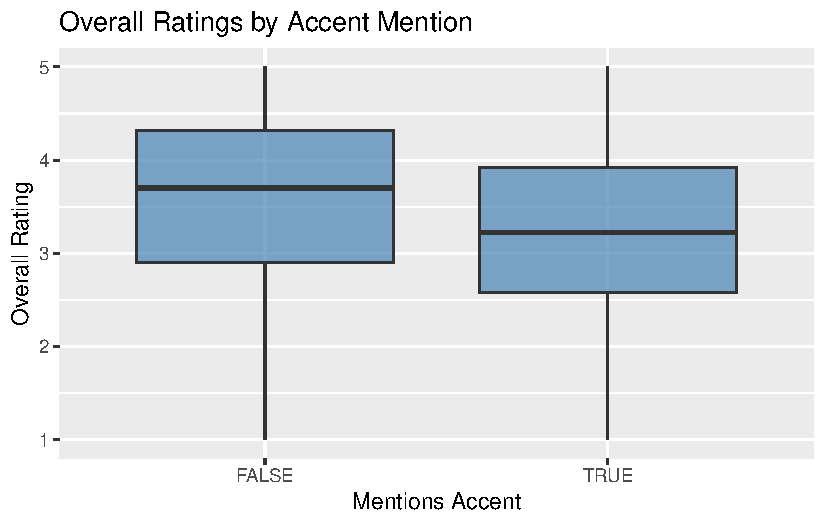
\includegraphics[keepaspectratio]{Lab07_files/figure-pdf/label - box plots-1.pdf}}

\subsubsection{Part d (Code: 1 pt)}\label{part-d-code-1-pt}

Using the \texttt{ggplot2} package, construct a set of histograms to
show the distribution of \texttt{overall} within each category. Play
around with the \texttt{center} and \texttt{binwidth} arguments until
you get a set of graphs where you have a good idea of the shape of the
distributions.

NOTE: Passing the argument \texttt{scales\ =\ "free\_y"} to
\texttt{facet\_wrap()} indicates to keep the x-axis fixed at 1-5 but
keep the y-axis free. This will allow us to compare shapes even if there
are many professors in one group and few professors in a different
group.

\paragraph{Solution}\label{solution-11}

\begin{Shaded}
\begin{Highlighting}[]
\FunctionTok{ggplot}\NormalTok{(RMP\_train,}
       \AttributeTok{mapping =} \FunctionTok{aes}\NormalTok{(}\AttributeTok{x =}\NormalTok{ overall)}
\NormalTok{       ) }\SpecialCharTok{+}
  \FunctionTok{geom\_histogram}\NormalTok{(}\AttributeTok{binwidth =} \FloatTok{0.25}\NormalTok{,}
                 \AttributeTok{fill =} \StringTok{"steelblue"}\NormalTok{,}
                 \AttributeTok{color =} \StringTok{"black"}\NormalTok{) }\SpecialCharTok{+}
  \FunctionTok{facet\_wrap}\NormalTok{(}\SpecialCharTok{\textasciitilde{}}\NormalTok{ mentions\_accent, }
             \AttributeTok{scales =} \StringTok{"free\_y"}
\NormalTok{             ) }\SpecialCharTok{+}
  \FunctionTok{labs}\NormalTok{(}
    \AttributeTok{title =} \StringTok{"Distribution of Overall Ratings by Accent Mention"}\NormalTok{,}
    \AttributeTok{x =} \StringTok{"Overall Rating"}\NormalTok{,}
    \AttributeTok{y =} \StringTok{"Count"}
\NormalTok{  )}
\end{Highlighting}
\end{Shaded}

\pandocbounded{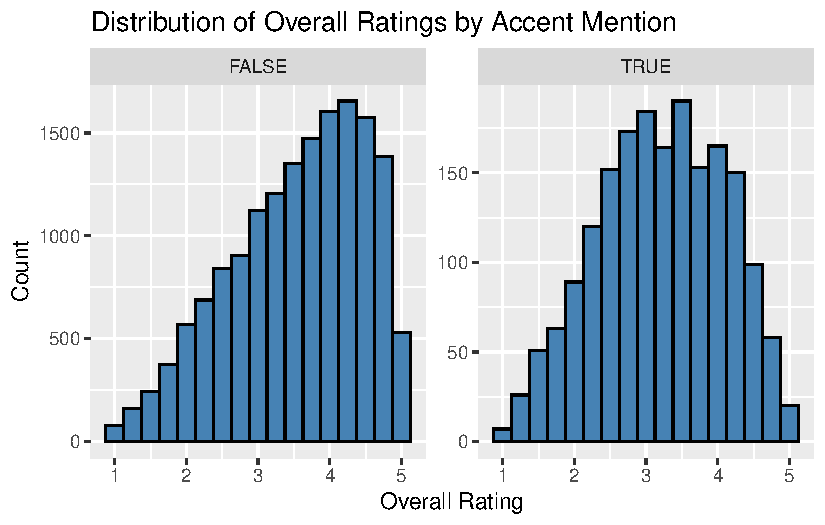
\includegraphics[keepaspectratio]{Lab07_files/figure-pdf/distributions of ratings by accent-1.pdf}}

\subsubsection{Part e (Explanation: 1
pt)}\label{part-e-explanation-1-pt}

Write 1-2 sentences describing anything interesting that you notice
based on your summaries, boxplots, and histograms. Again, try to address
the questions suggested at the beginning of Problem 2, and use similar
language to how you described what you expected.

\paragraph{Solution}\label{solution-12}

The distributions show that professors where students mention an accent
tend to have lower overall ratings compared to those where an accent is
not mentioned. The shape of the distributions looks fairly similar, but
the entire distribution for the TRUE group appears shifted downward.
This matches what I expected, since communication differences could
affect how students perceive the class. \#\# Problem 4: Beyond Two
Variables (2 pts total)

\subsubsection{Part a (Code: 1 pt)}\label{part-a-code-1-pt}

Update your scatterplot from Problem 2c to include your groups from
Problem 3 in different colors. You should also have a separate
regression line (or local regression curve) for each group.

\paragraph{Solution}\label{solution-13}

\begin{Shaded}
\begin{Highlighting}[]
\FunctionTok{ggplot}\NormalTok{(RMP\_train,}
       \AttributeTok{mapping =} \FunctionTok{aes}\NormalTok{(}\AttributeTok{x =}\NormalTok{ interest,}
                     \AttributeTok{y =}\NormalTok{ overall,}
                     \AttributeTok{color =}\NormalTok{ mentions\_accent)}
\NormalTok{       ) }\SpecialCharTok{+}
  \FunctionTok{geom\_point}\NormalTok{(}\AttributeTok{alpha =} \FloatTok{0.08}\NormalTok{) }\SpecialCharTok{+}
  \FunctionTok{geom\_smooth}\NormalTok{(}\AttributeTok{method =} \StringTok{"lm"}\NormalTok{,}
              \AttributeTok{se =} \ConstantTok{FALSE}\NormalTok{) }\SpecialCharTok{+}
  \FunctionTok{labs}\NormalTok{(}
    \AttributeTok{title =} \StringTok{"Interest vs Overall Rating by Accent Mention"}\NormalTok{,}
    \AttributeTok{x =} \StringTok{"Interest"}\NormalTok{,}
    \AttributeTok{y =} \StringTok{"Overall Rating"}\NormalTok{,}
    \AttributeTok{color =} \StringTok{"Mentions Accent"}
\NormalTok{  )}
\end{Highlighting}
\end{Shaded}

\begin{verbatim}
`geom_smooth()` using formula = 'y ~ x'
\end{verbatim}

\pandocbounded{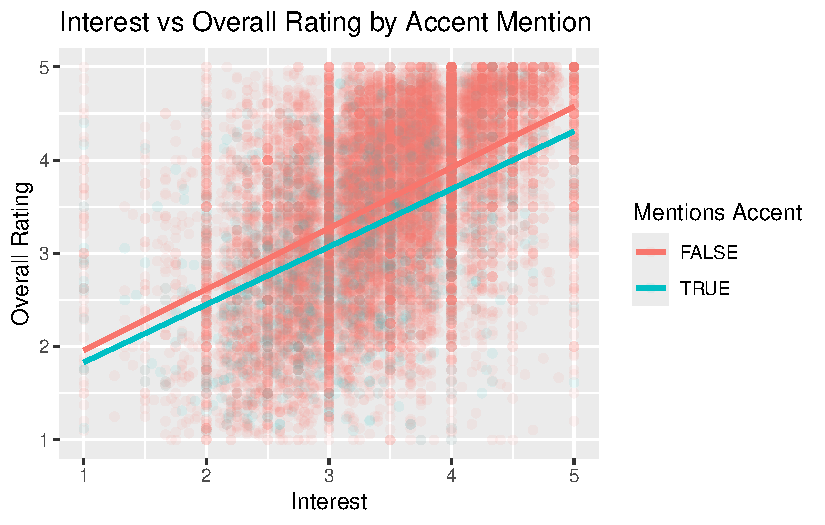
\includegraphics[keepaspectratio]{Lab07_files/figure-pdf/label - Interest overall by accent-1.pdf}}

\subsubsection{Part b (Explanation: 1
pt)}\label{part-b-explanation-1-pt}

Write 1-2 sentences describing anything interesting that you notice
based on your scatterplot. Generally, you want to think about how (if)
your answers to the questions from Problem 2 change depending on which
group you look at.

Again, try not to write with too much technical jargon.

It's very likely that with over 17,000 professors, this gets very messy.
If your scatterplot is just a blob, tell me that you can't see anything
useful.

\paragraph{Solution}\label{solution-14}

The positive relationship between interest and overall rating still
holds within both groups. However, the group where an accent is
mentioned consistently has lower overall ratings across all levels of
interest, since its regression line sits below the other one. The slopes
look fairly similar, but the TRUE group appears shifted downward
overall.




\end{document}
